\section{Ablations}
\label{section:ablations}


% \subsection{Action Set Prompt}
% \label{sec:action_pool}

The hyperparameters tuned for each ablation can be found in \Cref{appendix:hypers}.


\subsection{Action Set Prompt}
We assessed the impact of omitting the action embedding enumeration from the model context.
% The modified input to the model is:

% \[
% h_t = \left(o_{< t}, a^{emb}_{< t}, r_{< t}, o_t\right).
% \]

\Cref{table:ablations} reveals that removing the action set prompt did not significantly alter the number of unique actions attempted by each model. This suggests that models without the prompt continue to sample a diverse range of actions, comparable to the original setup. However, the presence of the prompt did affect the performance. We hypothesize that,
without the action set prompt, the model lacked explicit knowledge of the action space, which may have led to a more randomized sampling within the embedding space. Conversely, with the prompt in place, the model could directly target specific action embeddings.

The absence of the prompt was more detrimental in the Bernoulli Bandit environment, where each decision has a direct impact on the final outcome due to the environment's single-episode structure. However, in a multi-episode environment such as the Darkroom, the early lack of action space information becomes less impactful over time, as the model eventually encounters all actions through the context. This divergence highlights the prompt's critical role in enabling the model to make informed choices in environments where each option has immediate and lasting consequences. Note that the impact of action set prompt ablation on the performance got more pronounced as the number of arms grows.

% \Cref{fig:means_act_pool_ablation_num_acts} reveals that removing the action set prompt does not significantly alter the number of unique actions attempted by each model. This suggests that models without the prompt continue to sample a diverse range of actions, comparable to the original setup. However, as shown in \Cref{fig:means_act_pool_ablation}, the presence of the prompt does affect performance. We hypothesize that,
% % Our hypothesis as to why this is centers on the degree of control the model has over action selection. 
% without the action set prompt, the model lacks explicit knowledge of the action space, which may lead to a more randomized sampling within the embedding space. Conversely, with the prompt in place, the model can directly target specific action embeddings.

% \Cref{fig:means_act_pool_ablation} shows that the absence of the prompt is more detrimental in environments such as the Bernoulli Bandit, where each decision has a direct impact on the final outcome due to the environment's single-episode structure. However, in multi-episode environments such as the Darkroom, the early lack of action space information becomes less impactful over time, as the model eventually encounters all actions through the context. This divergence highlights the prompt's critical role in enabling the model to make informed choices in environments where each option has immediate and lasting consequences. Note that, as one can see in \Cref{fig:bandit_act_pool_ablation}, the impact of action set prompt ablation on the performance gets more pronounced as the number of arms grows.

% \subsection{Contrastive Loss}


\subsection{Contrastive Loss}
In principle, the prediction of action embedding can be facilitated by various ways. Here, we considered the performance of a model that was asked to directly copy the corresponding embedding from its context to the output. To achieve it, we used mean squared error (MSE) loss instead of contrastive loss.

In this case, probabilistic interpretation became less meaningful, which is why the nearest neighbor of the predicted vector was chosen as an action index, without sampling.

% \begin{figure*}[t!]
%     \vskip 0.2in
%     \centering
%     \begin{subfigure}{\columnwidth}
%         \centering
%         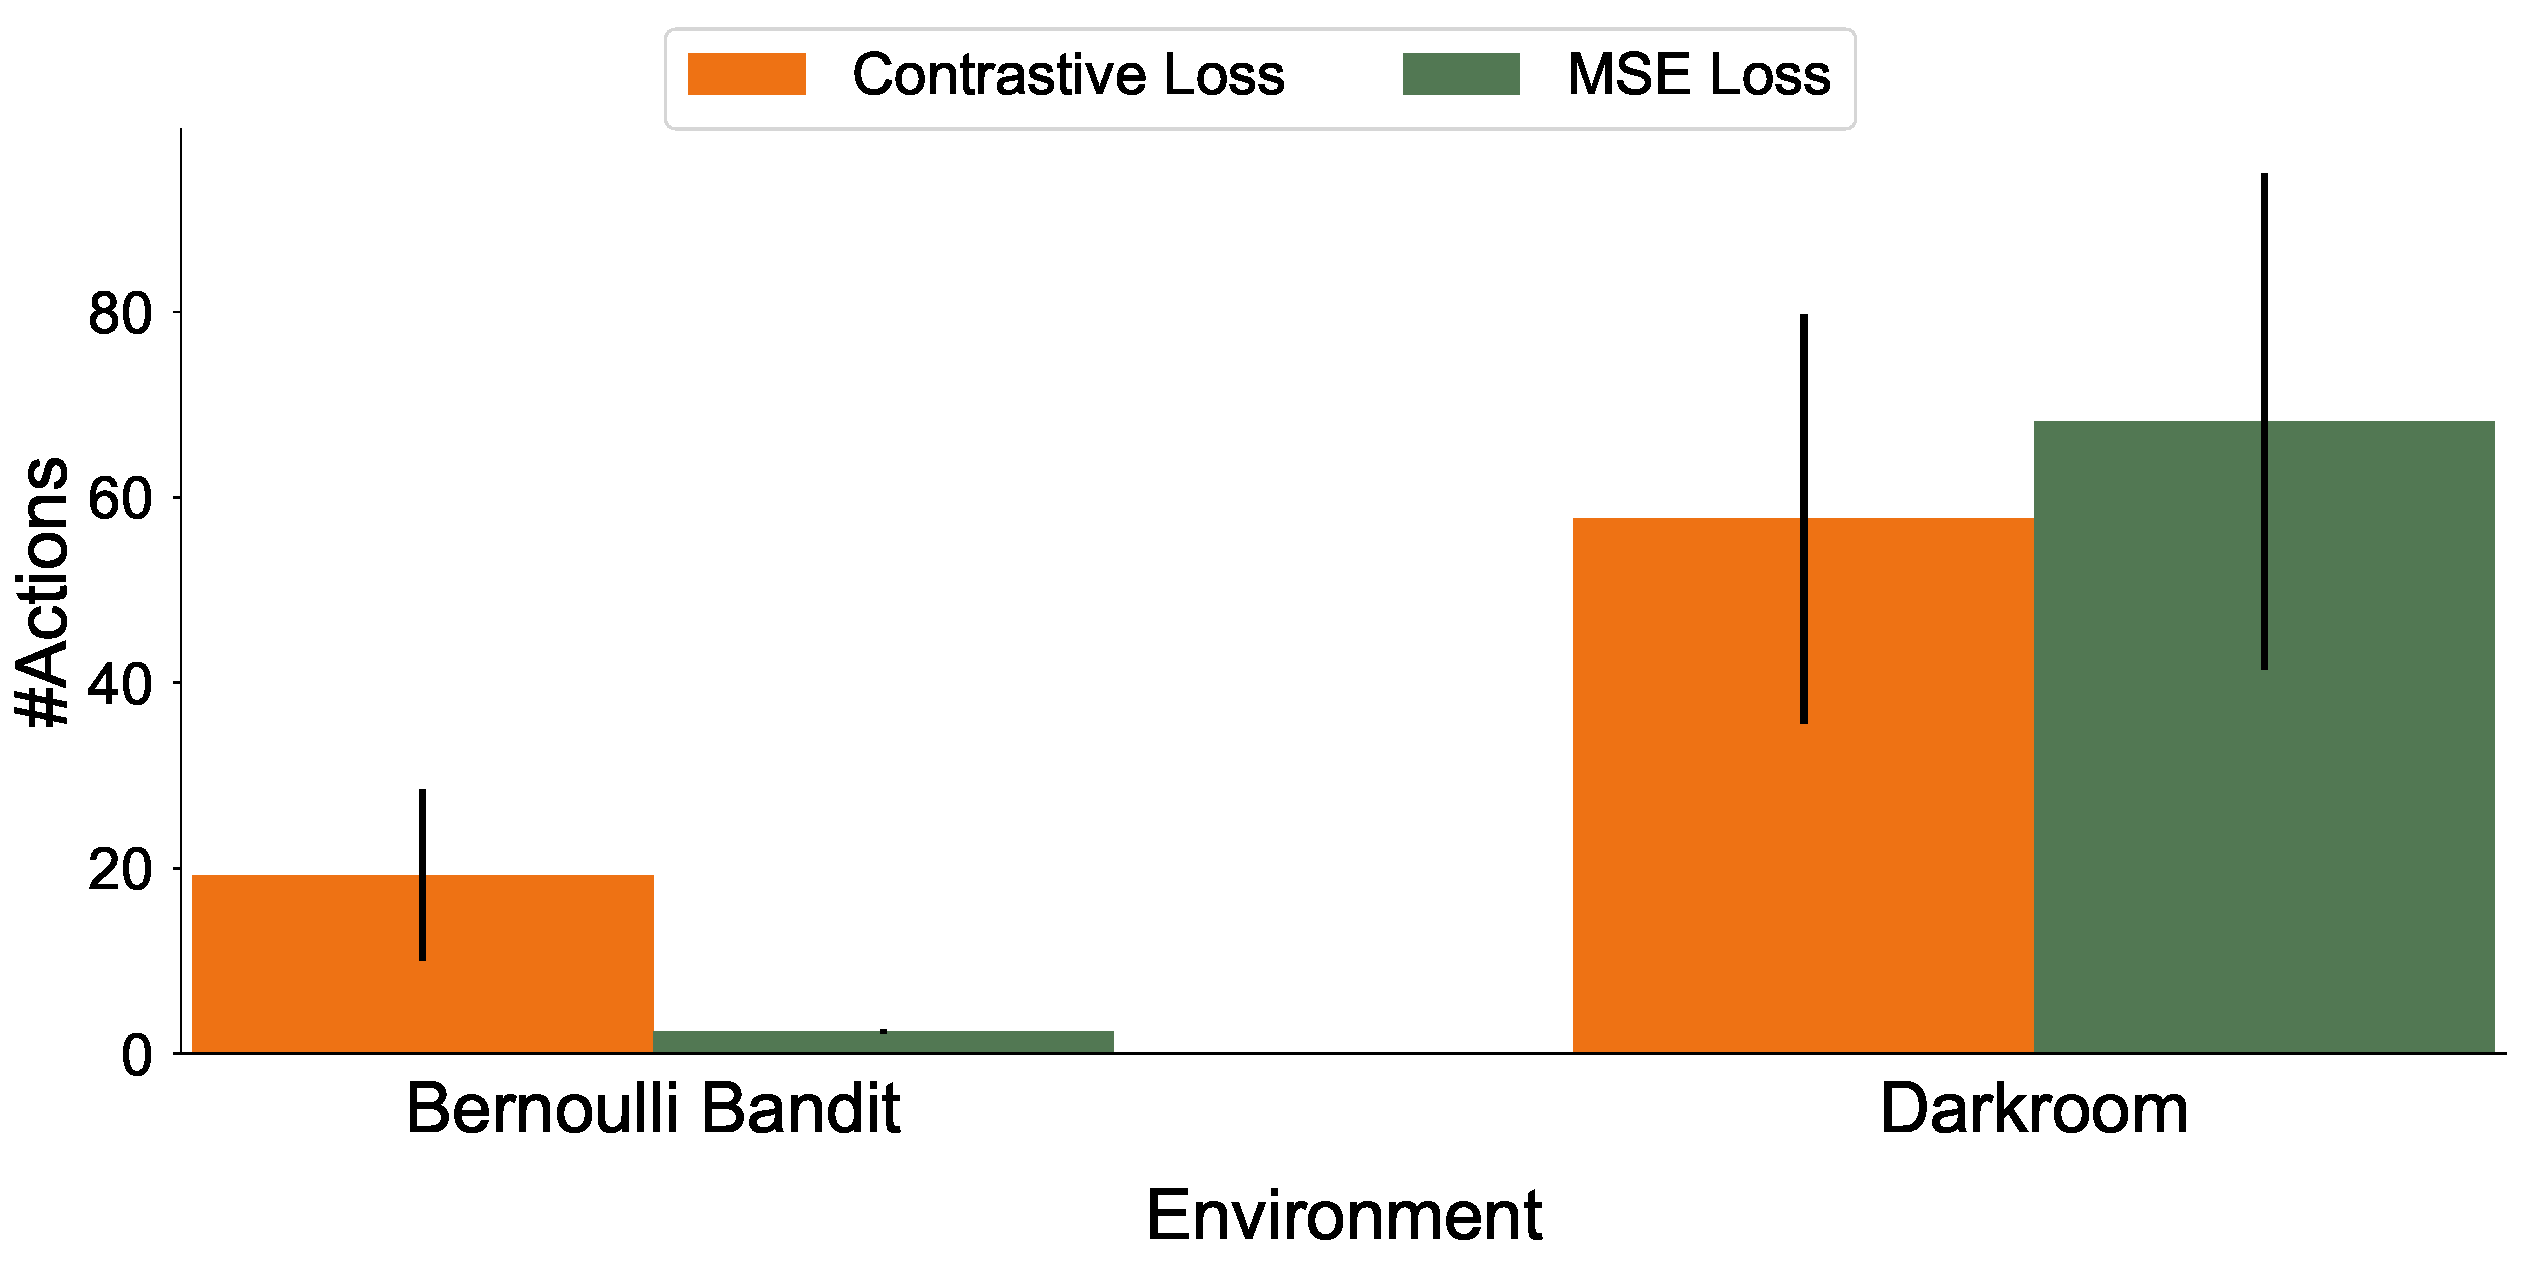
\includegraphics[width=0.85\columnwidth]{images/means_mse_ablation_num_acts.pdf}
%         % 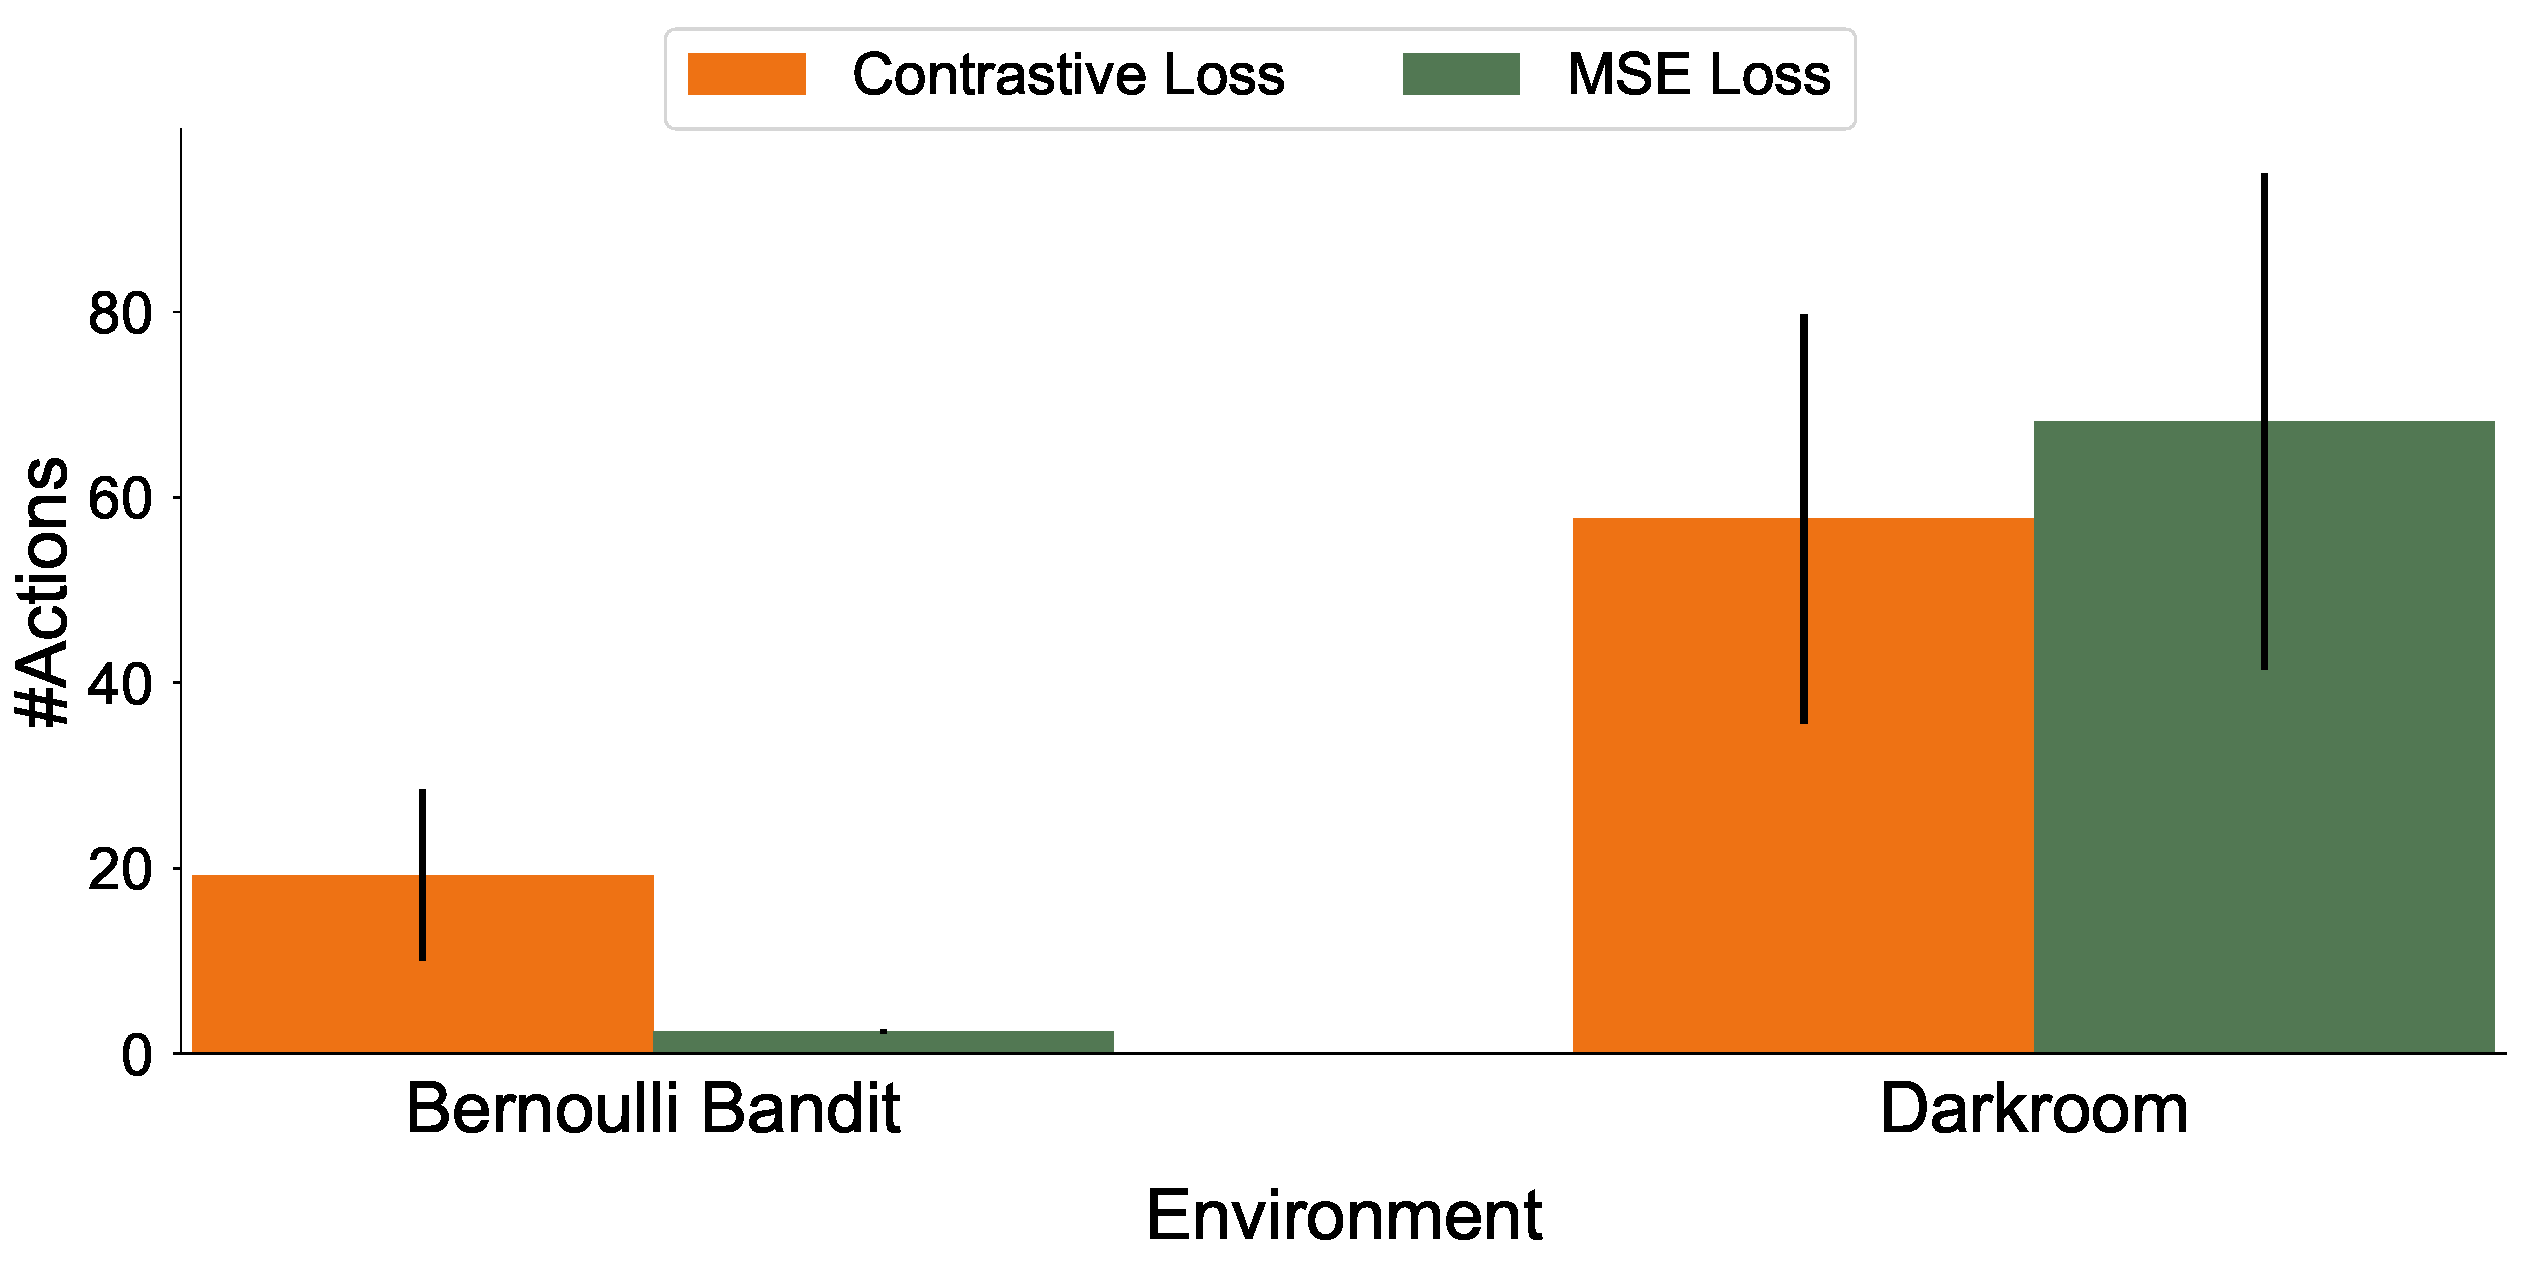
\includegraphics[width=0.45\columnwidth]{images/means_mse_ablation_num_acts.pdf}
%         \caption{}
%         \label{fig:means_mse_ablation_num_acts}
%     \end{subfigure}
%     ~
%     % \hfill
%     \begin{subfigure}{\columnwidth}
%         \centering
%         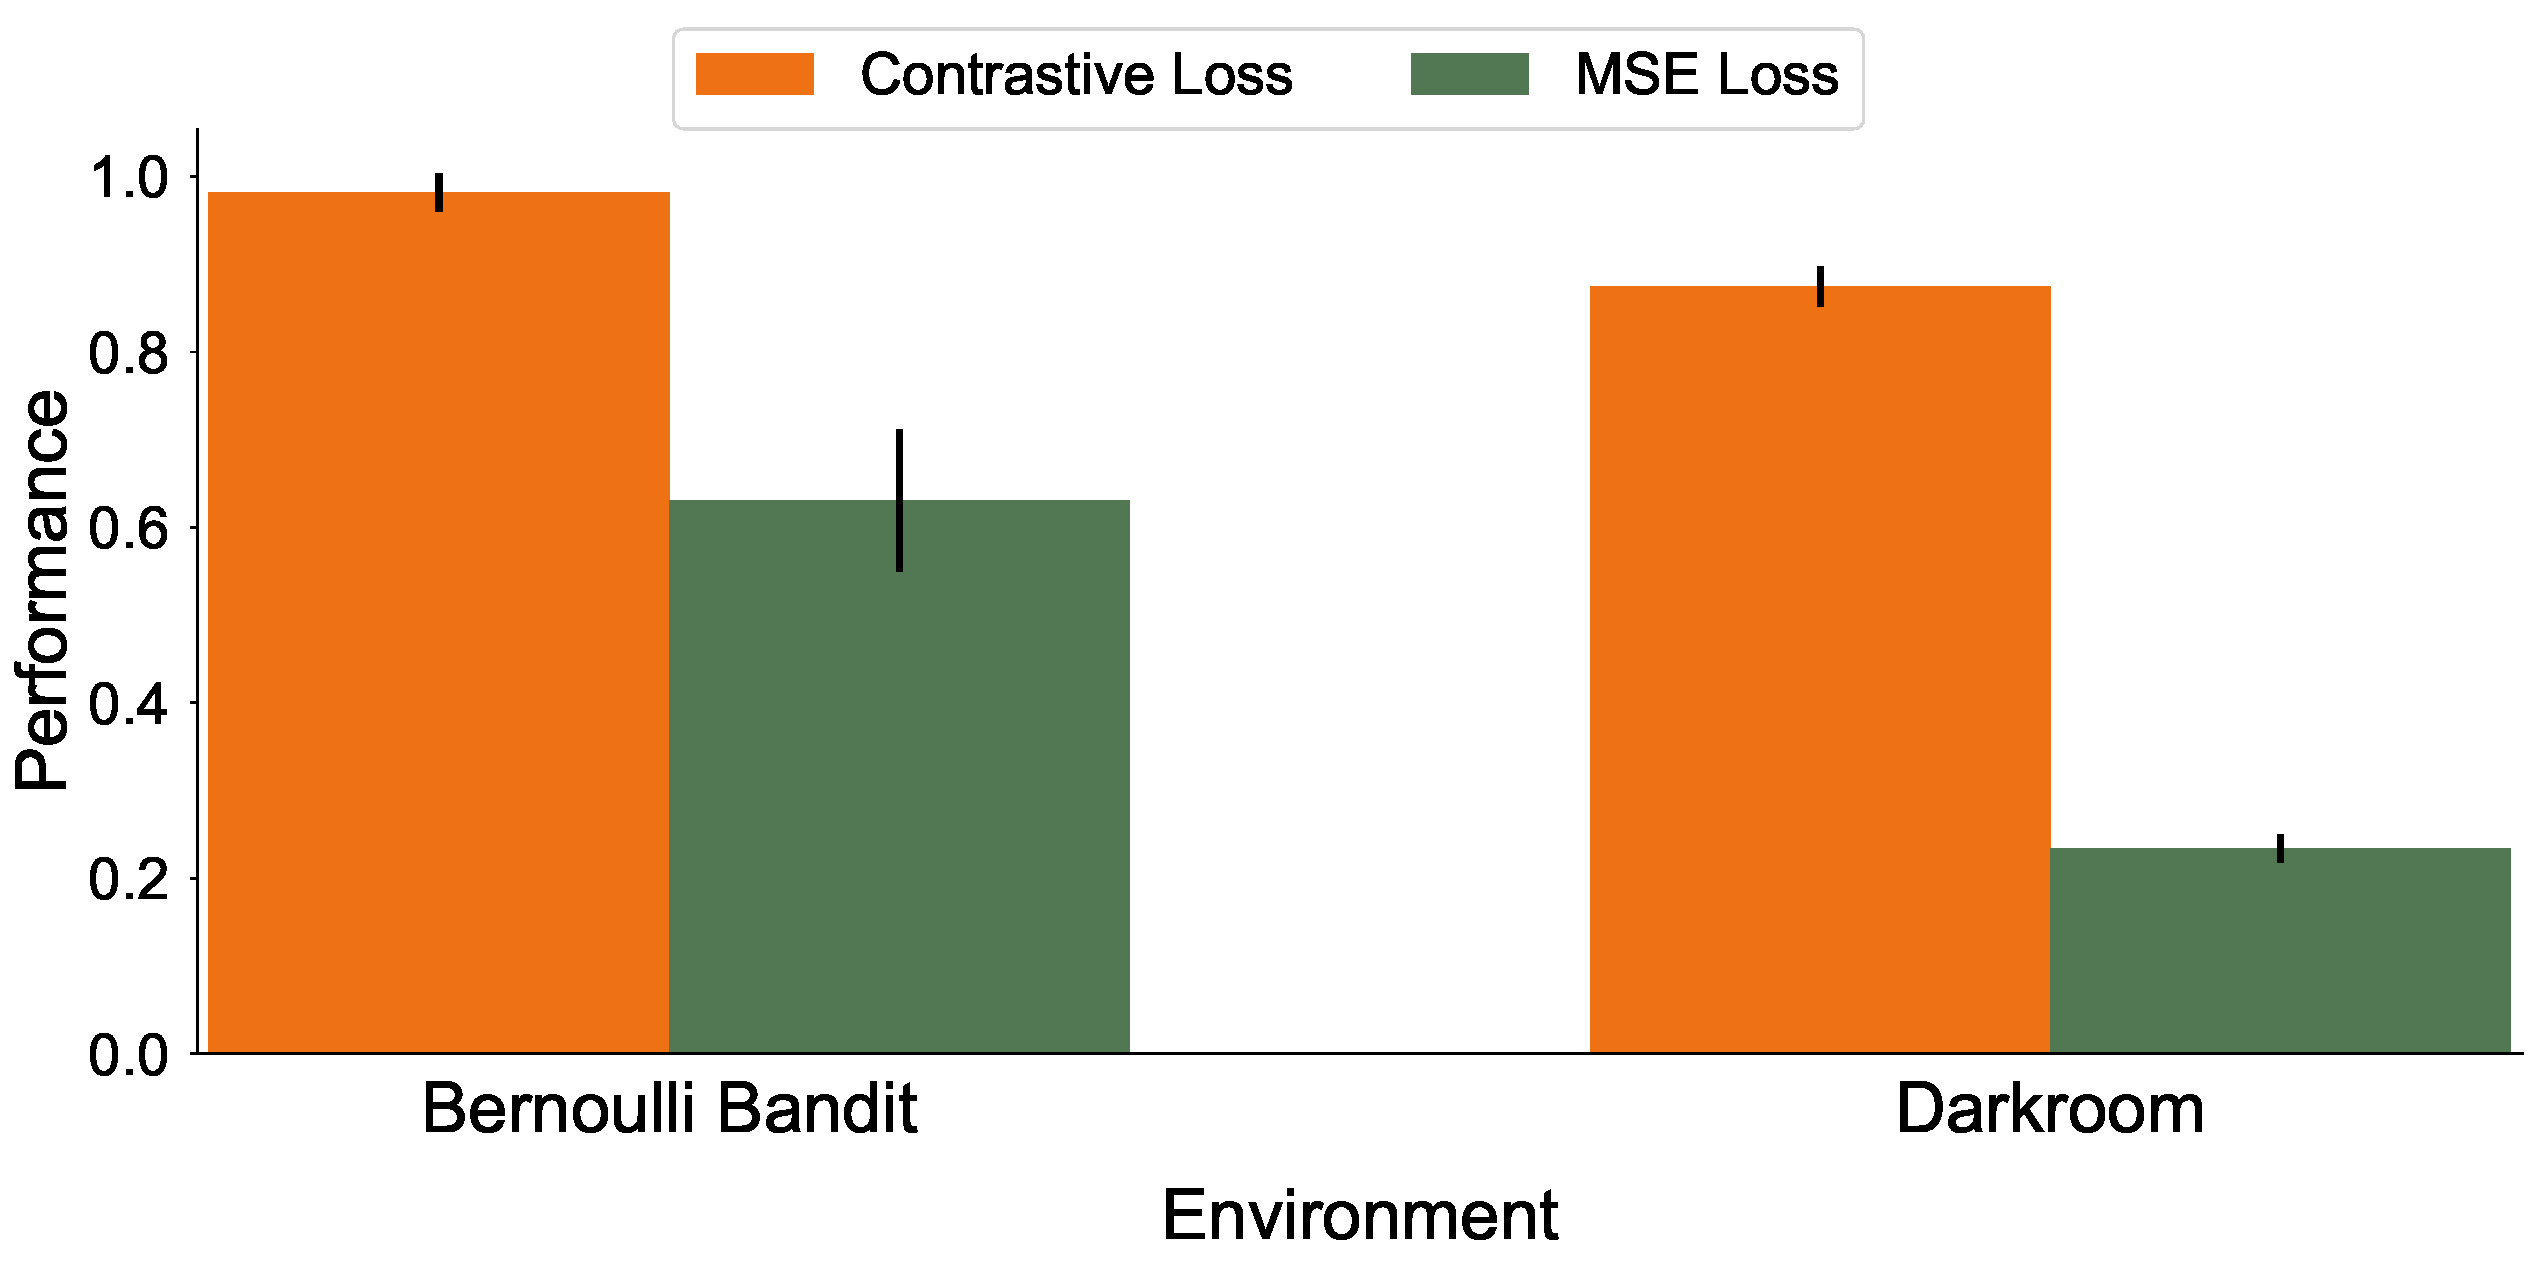
\includegraphics[width=0.85\columnwidth]{images/means_mse_ablation.pdf}
%         % 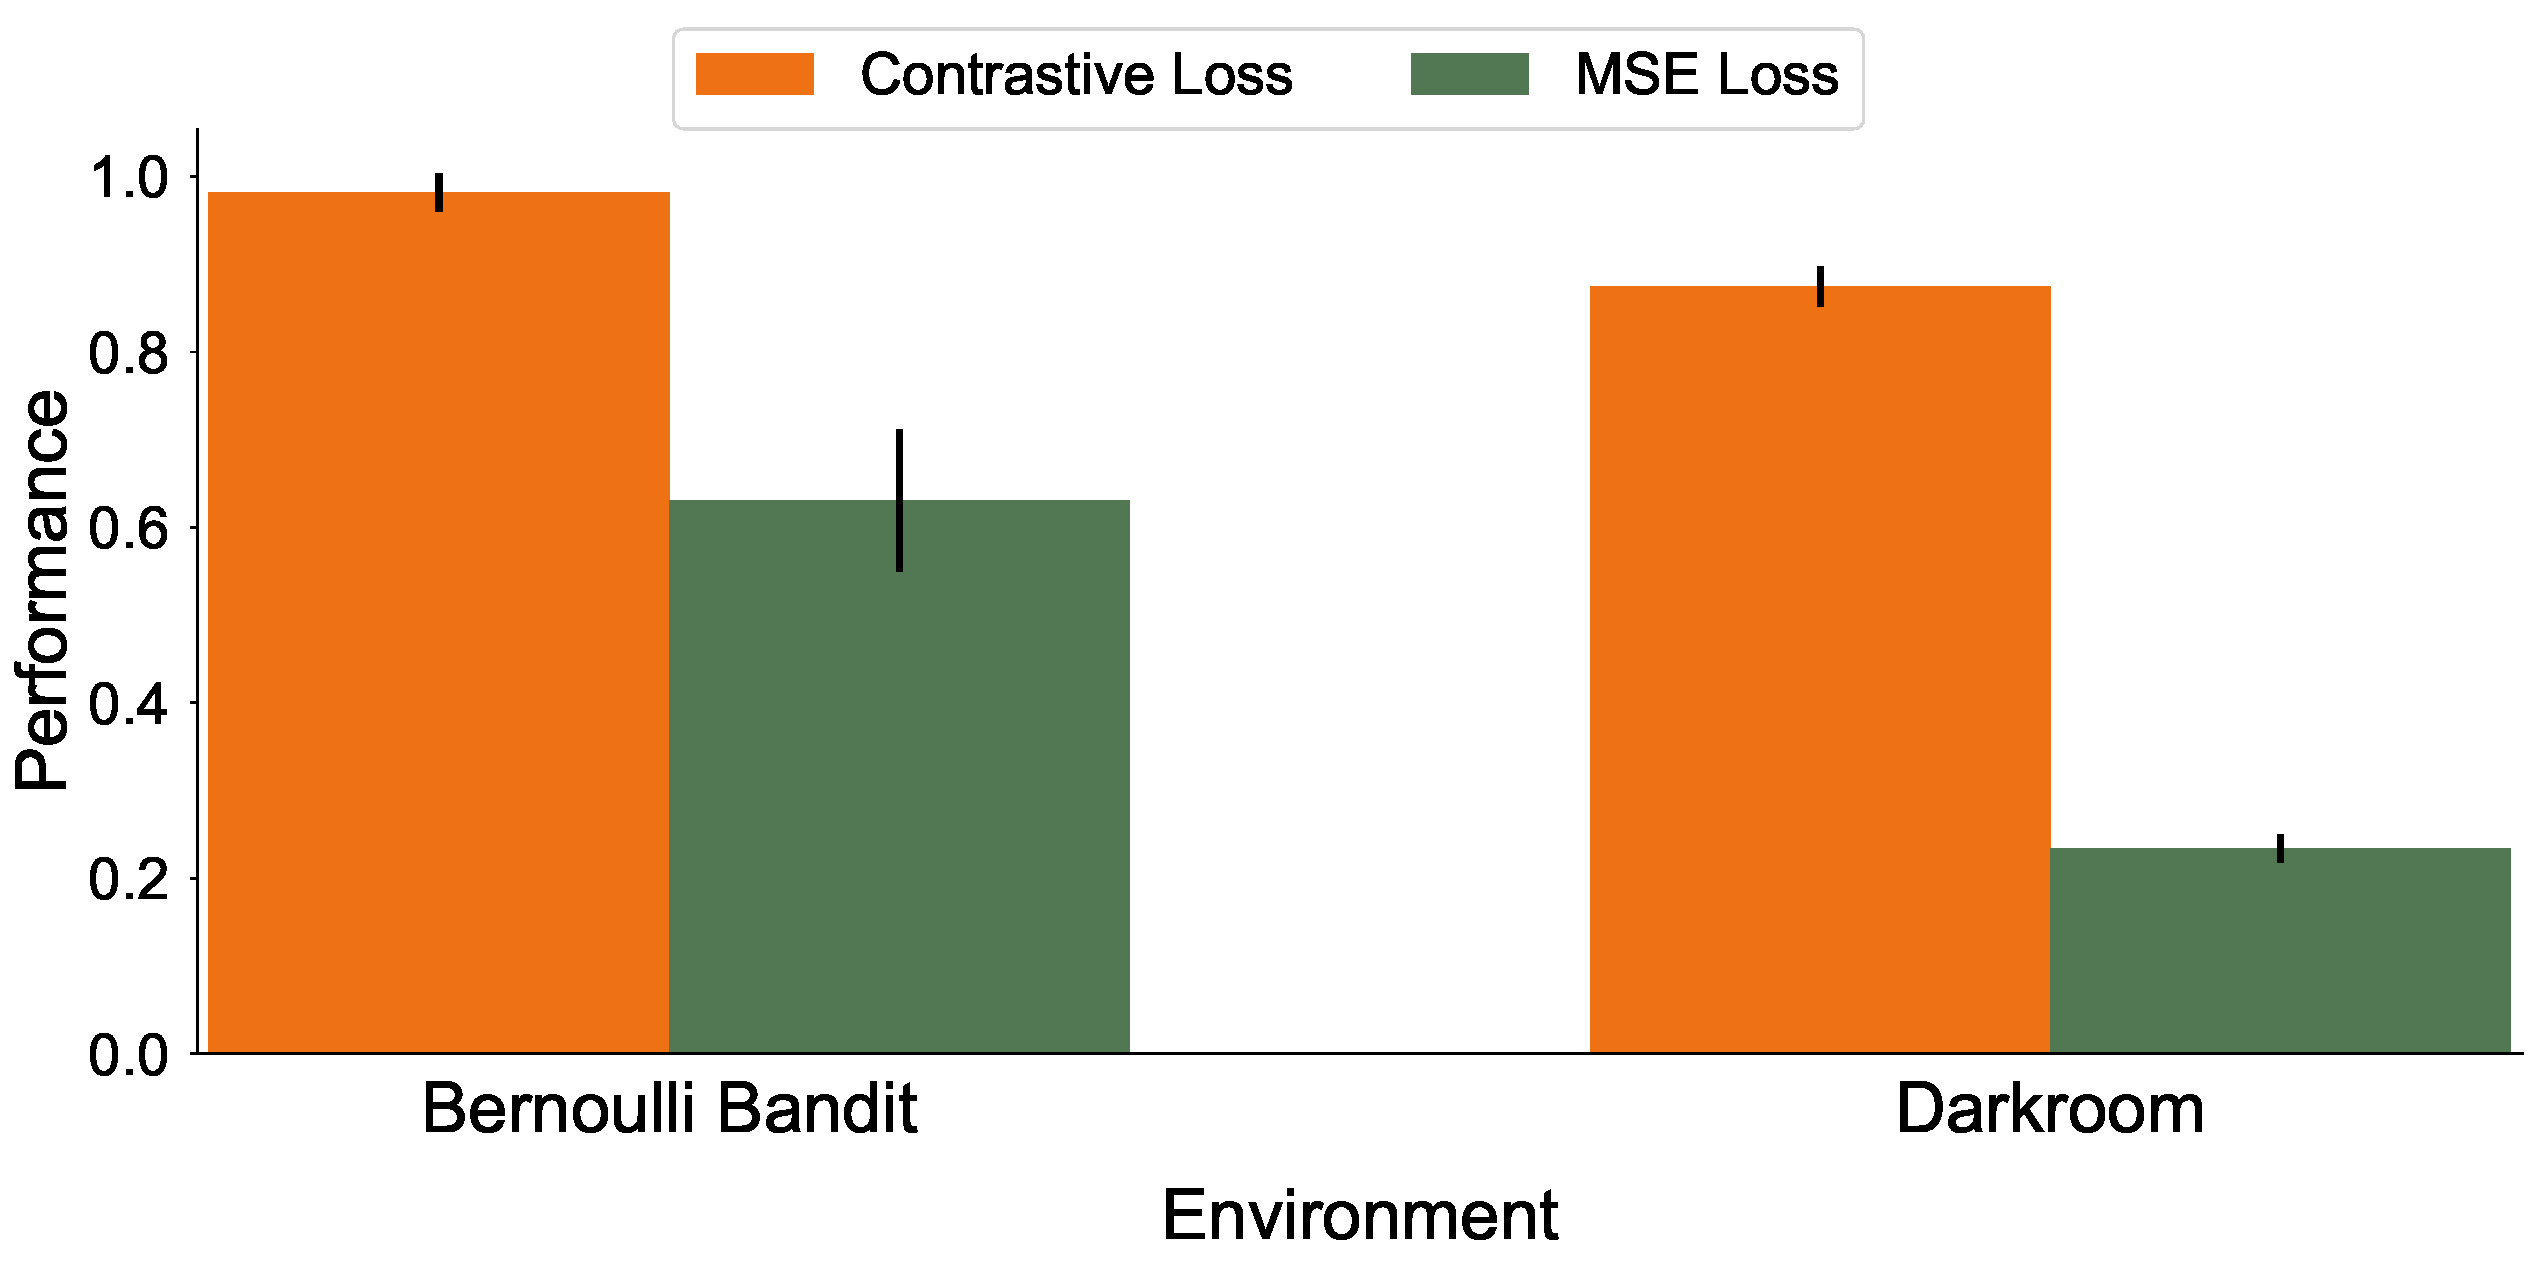
\includegraphics[width=0.45\columnwidth]{images/means_mse_ablation.pdf}
%         \caption{}
%         \label{fig:means_mse_ablation}
%     \end{subfigure}
%     \caption{\textbf{Evaluating the Effectiveness of Contrastive vs. MSE Loss:} This figure presents a comparative analysis of contrastive loss and mean squared error (MSE) loss on the training efficiency and performance metrics of our model. All results are averaged across various action sets within their respective environments and are based on data from five distinct training seeds. \textit{Performance} on the y-axis represents the normalized regret for the Bernoulli Bandit environment, and the success rate for Darkroom. \textbf{(a)} depicts the impact on the model's ability to explore: in the Bernoulli Bandit environment, the model trained with MSE loss exhibits a limited exploration range, focusing on only a small subset of the available actions. Conversely, on the Darkroom environment there is a slight increase in the number of actions attempted. \textbf{(b)} Regardless of how the MSE loss affects the amount of actions used, the final performance of the model on both environments drops significantly.
%     }
%     \vskip -0.2in
% \end{figure*}

\Cref{table:ablations} illustrates a significant decline in the variety of actions attempted by the model under this configuration within the bandit environment, showing that the model concentrated only on a fraction of the action set. Though the final regrets for this model were far from random, we point out that this result is because the model skipped exploration phase and went directly to an exploitation of suboptimal actions. That allowed it not to waste time on even more suboptimal ones via exploration. \Cref{appendix:mse_headless_curves} shows the in-context curves of both models, providing more insight into MSE's effect on model quality.

Conversely, on the Darkroom environment, the loss substitution led to a marginal increase in the amount of attempted actions. However, this did not lead to an increased performance. In fact, the performance of this model on the Darkroom environment was similar to a random behavior. 

In summary, although the employed neural network architecture was capable of learning an improvement operator and demonstrating ICL capabilities, the implemented loss function played a crucial role in the success of this learning process. We emphasize the importance of our design choice to use contrastive loss by showing that a more naive approach of directly copying the action embeddings, as incentivized by MSE loss, resulted in underperformance.

% \Cref{fig:means_mse_ablation_num_acts} illustrates a significant decline in the variety of actions attempted by the model under this configuration within the bandit environment, showing that the model concentrates only on a fraction of the action set. \textcolor{blue}{Though the final regrets for this model are far from random, as depicted in \Cref{fig:means_mse_ablation}, we point out that this result is because the model skips exploration phase and goes directly to an exploitation of suboptimal actions. That allows it not to waste time on even more suboptimal ones via exploration. \Cref{appendix:mse_headless_curves} shows the in-context curves of both models, providing more insight into MSE's effect on model quality.}

% Conversely, on the Darkroom environment, the loss substitution leads to a marginal increase in the amount of attempted actions. However, as one can see in \Cref{fig:means_mse_ablation}, this does not lead to increased performance. In fact, the performance of this model on the Darkroom environment is similar to random behavior. 

% In summary, although the employed neural network is capable of learning an improvement operator and demonstrating ICL capabilities, the implemented loss function plays a crucial role in the success of this learning process. We emphasize the importance of our design choice to use contrastive loss by showing that a more naive approach of directly copying the action embeddings, as incentivized by MSE loss, results in underperformance.

\subsection{Orthonormal Action Embeddings}
In this ablation study, we underscored the significance of employing orthonormal vectors for action embeddings by contrasting them with vectors derived from a standard normal distribution. Our preference for the former stemmed from their ability to simplify the approximation of action probabilities because of their property of independence. Unlike embeddings from a standard normal distribution, orthonormal vectors ensure that assigning a probability weight to one vector does not unintentionally influence another (we illustrate it in \Cref{appendix:act_emb_dependence}). This concept echoes the principle of \textit{superposition}, observed when models incorporate more features than available dimensions, leading to feature interference \cite{elhage2022superposition}.

\Cref{table:ablations} illustrates the consequences of using linearly dependent action embeddings, manifesting as diminished performance across Bernoulli bandits and Darkroom scenarios. Notably, these results bear a striking resemblance to "Prompt Ablation", with both indicating a slight performance dip in Darkroom, a more noticeable decline in Bernoulli Bandits, and a general downtrend as the number of bandit arms grows. This parallel underscores a shared objective between these design choices: refining the model's capacity for precise action selection.

% \textcolor{blue}{\textbf{Orthonormal Action Embeddings:}}
% \textcolor{blue}{In this ablation study, we underscore the significance of employing orthonormal vectors for action embeddings by contrasting them with vectors derived from a standard normal distribution. Our preference for the former stems from their ability to simplify the approximation of action probabilities, a benefit directly attributable to their property of independence. Unlike embeddings from a standard normal distribution, orthonormal vectors ensure that assigning a probability weight to one vector does not unintentionally influence another. This concept echoes the principle of "superposition", observed when models incorporate more features than available dimensions, leading to feature interference \citep{elhage2022superposition}.}

% \textcolor{blue}{We illustrate this principle through an analysis of cosine similarities between action embeddings, comparing orthonormal vectors to those from a standard normal distribution (see \Cref{appendix:act_emb_dependence}). The analysis reveals non-zero cosine similarities for the standard normal distribution, indicating that a vector perfectly aligned with one action embedding may erroneously attribute non-zero probabilities to other actions.}

% \textcolor{blue}{\Cref{fig:act_emb_ablation} illustrates the consequences of using linearly dependent action embeddings, manifesting as diminished performance across Bernoulli bandits and Darkroom scenarios. Notably, this figure bears a striking resemblance to \Cref{fig:act_set_prompt_ablation}, with both indicating a slight performance dip in Darkroom, a more noticeable decline in Bernoulli Bandits, and a general downtrend as the number of bandit arms grows. This parallel underscores a shared objective between these design choices: refining the model's capacity for precise action selection.}

% \begin{figure*}[t]
%     \vskip 0.2in
%     \centering
%     \begin{subfigure}{\columnwidth}
%         \centering
%         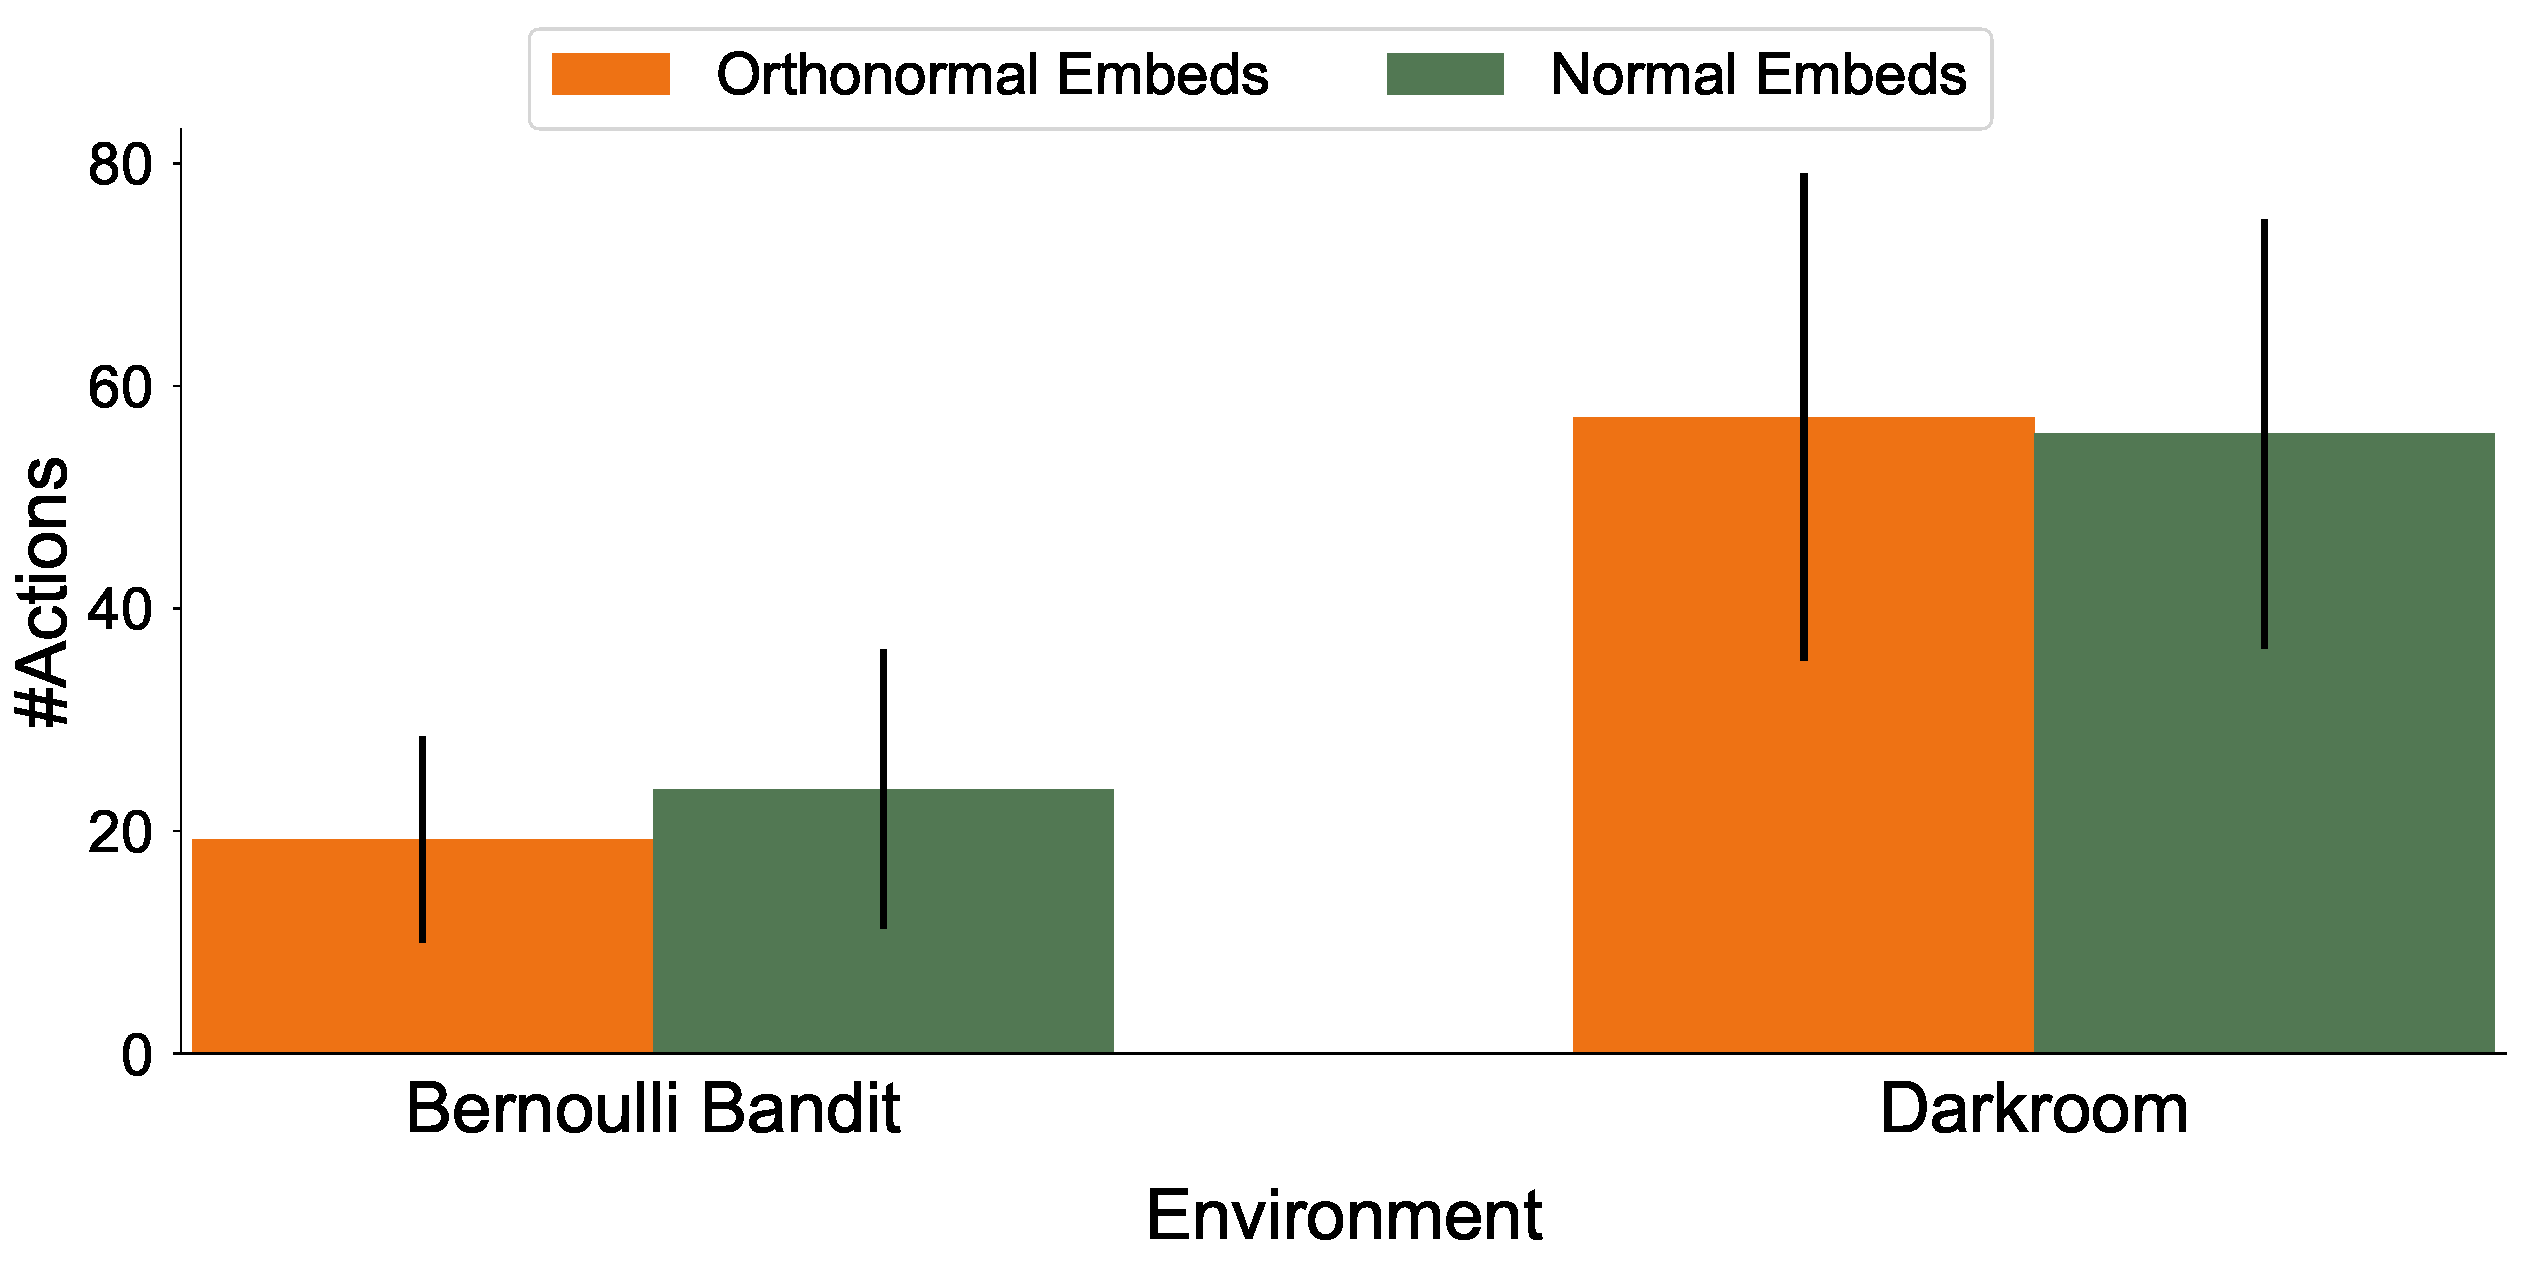
\includegraphics[width=0.85\columnwidth]{images/means_embed_ablation_num_acts.pdf}
%         \caption{}
%         \label{fig:means_embed_ablation_num_acts}
%     \end{subfigure}
%     ~
%     \begin{subfigure}{\columnwidth}
%         \centering
%         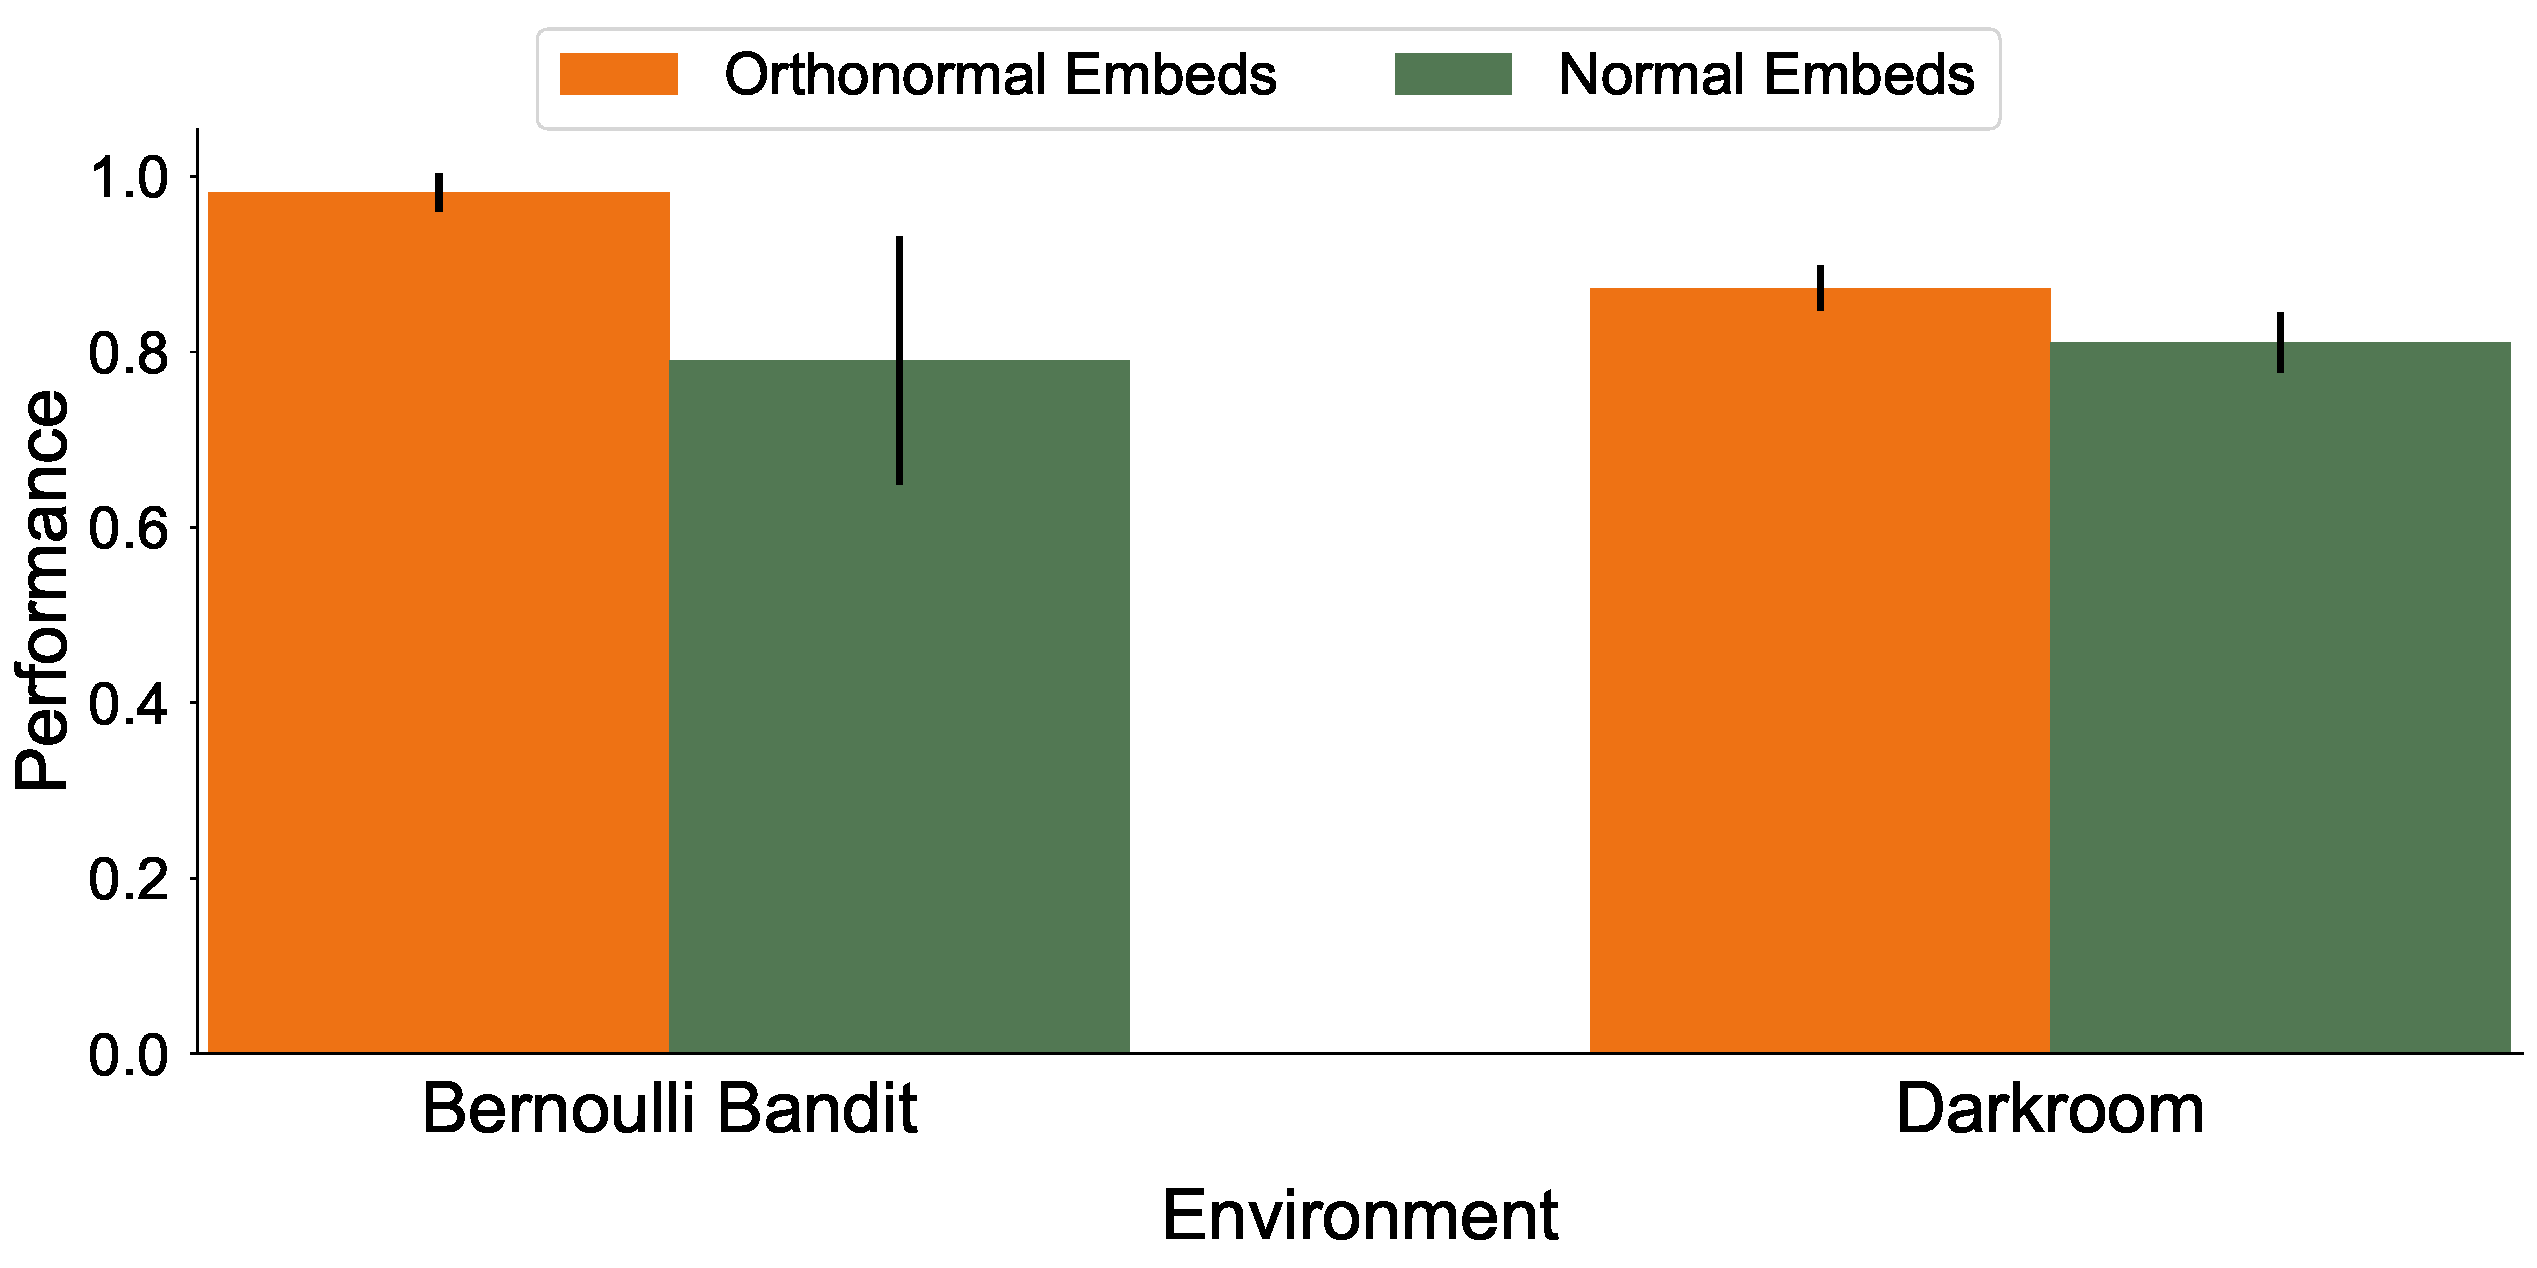
\includegraphics[width=0.85\columnwidth]{images/means_embed_ablation.pdf}
%         \caption{}
%         \label{fig:means_embed_ablation}
%     \end{subfigure}
%     \vfill
%     \begin{subfigure}{\textwidth}
%         \centering
%         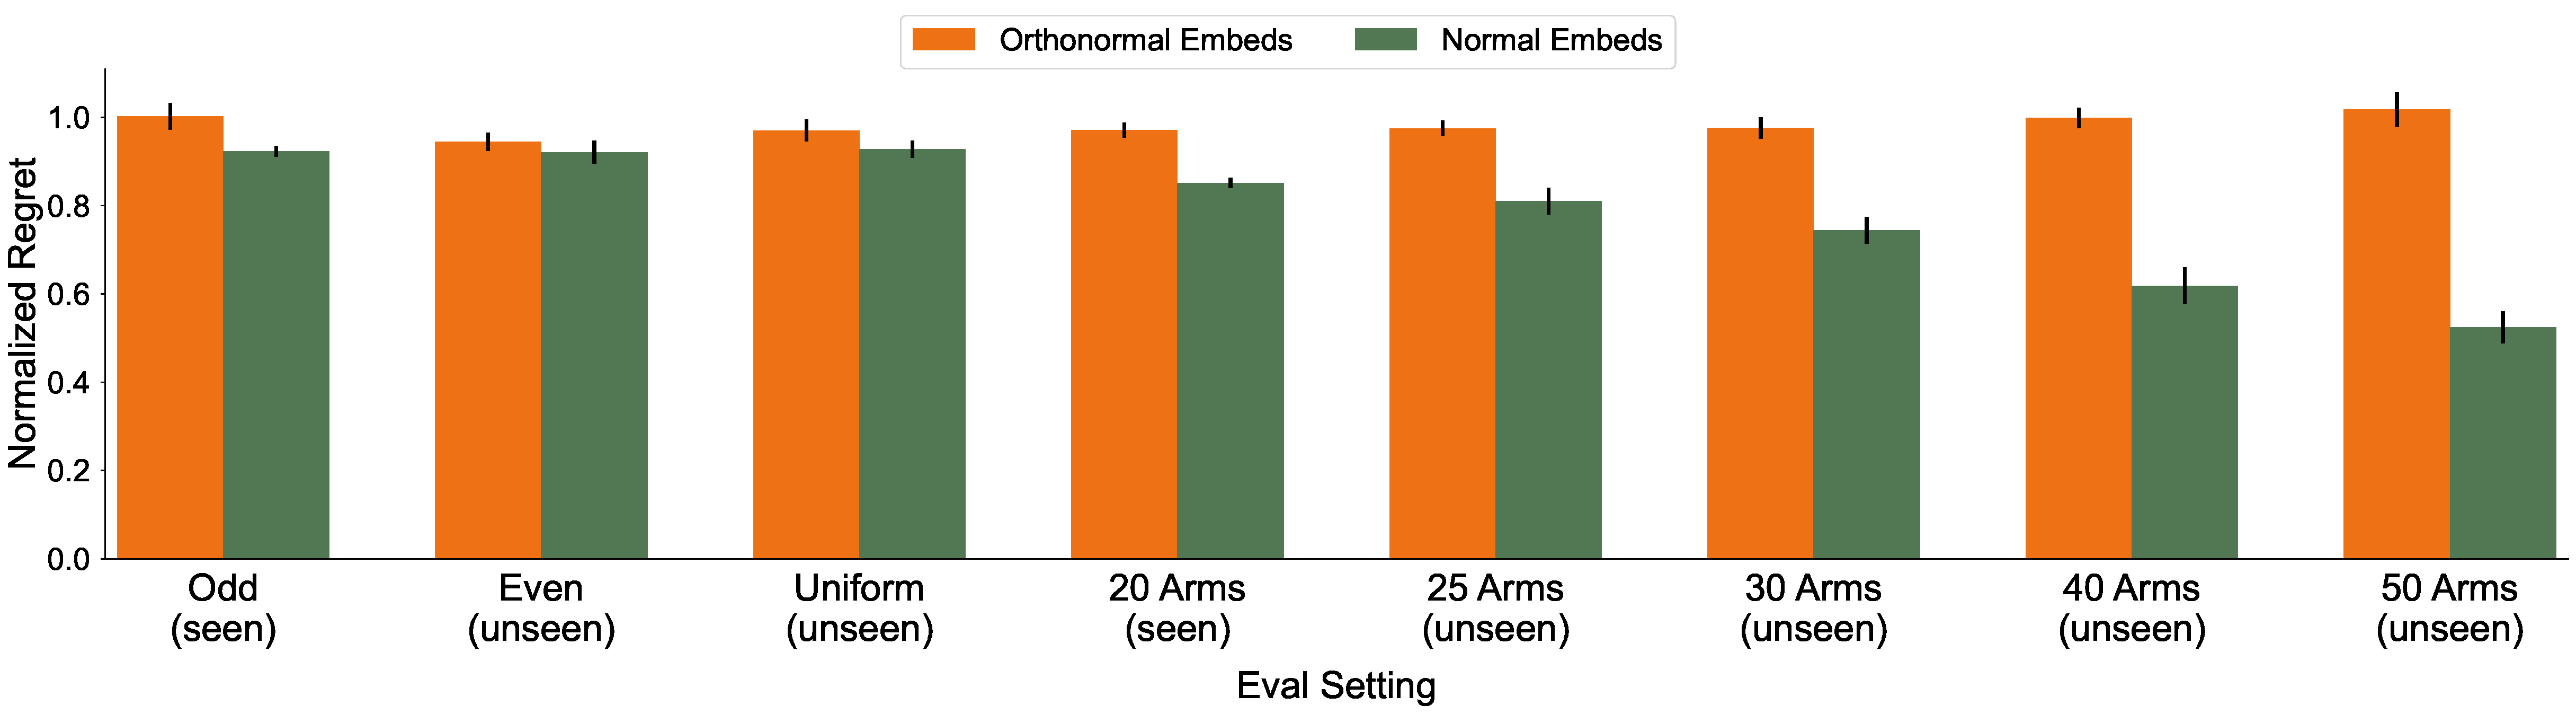
\includegraphics[width=0.95\textwidth]{images/bandit_embed_ablation.pdf}
%         \caption{}
%         \label{fig:bandit_embed_ablation}
%     \end{subfigure}
%     \caption{\textcolor{blue}{\textbf{Impact of Action Embedding Distribution:} (a) The type of action embedding distribution minimally affects the variety of actions explored by agents, as seen in averaged action counts across sets. (b) Distribution type significantly influences performance in environments like the Bernoulli Bandit (measured by normalized regret) but less so in Darkroom (measured by success rate). This shows through average performance across action sets. (c) As the action space grows, the choice of action embedding distribution becomes more critical, suggesting that larger numbers of correlated embeddings can hinder performance.}}
%     \label{fig:act_emb_ablation}
%     \vskip -0.2in
% \end{figure*}
